\documentclass{article}

\usepackage{arxiv}
\usepackage{amsmath}
\usepackage[utf8]{inputenc}
\usepackage[T1]{fontenc}
\usepackage{hyperref}
\usepackage{url}
\usepackage{booktabs}
\usepackage{amsfonts}
\usepackage{nicefrac}
\usepackage{microtype}
\usepackage{multirow}
\usepackage{cleveref}
\usepackage{listings}
\usepackage{graphicx}
\usepackage{natbib}
\usepackage{float}
\usepackage{enumitem}

\title{Rapport final}

\newif\ifuniqueAffiliation
\uniqueAffiliationtrue

\author{\hspace{1mm}Alexandre Eberhardt\\
	Master of Computer Science\\
	Laval University\\
	Québec, QC \\
	\texttt{alexandre.eberhardt.1@ulaval.ca} \\
	\And
    \hspace{1mm}Rémi Hercouët \\
	Master of Computer Science\\
	  Laval University\\
	Québec, QC \\
	\texttt{remi.hercouet.1@ulaval.ca} \\
}

\renewcommand{\headeright}{}
\renewcommand{\undertitle}{}
\renewcommand{\shorttitle}{Rapport Final - IFT-7201}

\hypersetup{
pdftitle={Rapport final},
pdfauthor={Alexandre Eberhardt, Rémi Hercouët},
}

\begin{document}
\maketitle
\vspace{-0.5cm}

\begin{center}
    Code source du projet : \url{https://github.com/alexandreeberhardt/RL-FrozenLake}
\end{center}

% =============================================================================
\section{Cas d'étude}
% =============================================================================

\subsection{Description de l'environnement}

L'environnement \href{https://gymnasium.farama.org/environments/toy_text/frozen_lake/}{Frozen Lake}~\citep{towers2024gymnasium} de la bibliothèque Gymnasium modélise un processus de décision markovien (MDP) dans lequel un agent doit traverser un lac gelé.

\textbf{États et actions.} L'espace d'états est discret : chaque état $s \in \{0, \ldots, N^2{-}1\}$ correspond à la position de l'agent dans une grille $N \times N$ (numérotée ligne par ligne, de gauche à droite). L'espace d'actions est également discret : $\mathcal{A} = \{0, 1, 2, 3\}$ correspondant respectivement aux directions gauche, bas, droite et haut.

\textbf{Paramètres configurables.} La \textbf{carte} est définie par une matrice de tuiles (S : départ, F : glace, H : trou, G : objectif), dont le nombre et le positionnement des tuiles H sont entièrement personnalisables. La \textbf{stochasticité} est contrôlée par le paramètre \textit{success\_rate} : avec probabilité \textit{success\_rate}, l'agent se déplace dans la direction souhaitée ; sinon il glisse perpendiculairement. Enfin, la \textbf{distribution des récompenses} associe une valeur scalaire à chaque type de tuile d'arrivée (H, G, F).

\subsection{Nos cas d'études}

Trois cas d'étude ont été conçus pour isoler des défis distincts. Chaque environnement est instancié via \texttt{gym.make('FrozenLake-v1', desc=..., is\_slippery=True, success\_rate=..., reward\_schedule=...)}.

\textbf{Cas 1 — Efficacité pure.} Grille 7$\times$7 clairsemée (3~trous isolés). L'objectif est d'apprendre le chemin le plus court. La pénalité par pas ($-0.01$) pousse l'agent vers les trajectoires courtes sans rendre l'environnement dangereux. Paramètres : \textit{success\_rate}$=0.9$, récompenses $\{G:+1.0,\ H:-0.5,\ F:-0.01\}$.

\textbf{Cas 2 — Évitement strict.} Un unique couloir diagonal praticable, entièrement entouré de trous. Toute glissade hors du couloir est fatale. L'enjeu est la survie, pas l'efficacité. Paramètres : \textit{success\_rate}$=0.9$, récompenses $\{G:+1.0,\ H:-1.0,\ F:0.0\}$.

\textbf{Cas 3 — Compromis risque/récompense.} Deux chemins vers l'objectif : un chemin court (6~pas le long de la première ligne, risqué car la glissade vers le bas mène directement aux trous) et un chemin long ($\approx$18~pas par contournement, sûr mais coûteux). La pénalité par pas élevée ($-0.05$) et la forte récompense à l'objectif ($+1.75$) créent une tension entre vitesse et sécurité. Paramètres : \textit{success\_rate}$=0.75$, récompenses $\{G:+1.75,\ H:-1.0,\ F:-0.05\}$.

\begin{figure}[htbp]
    \centering
    \begin{minipage}{0.32\textwidth}
        \centering
        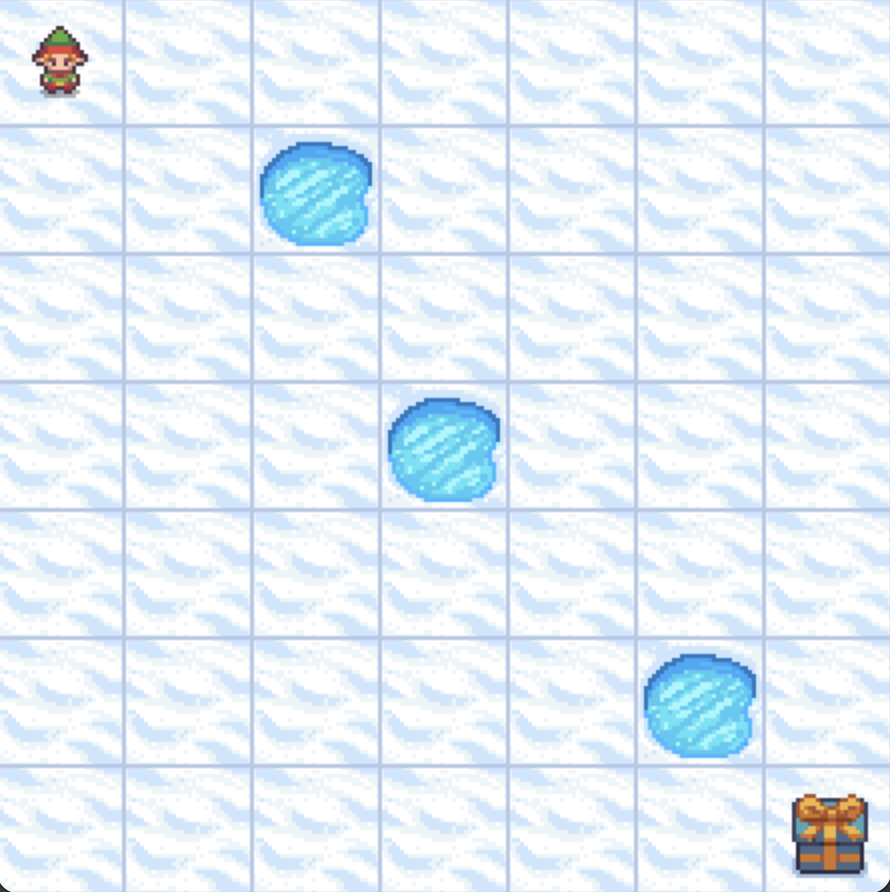
\includegraphics[width=0.8\linewidth]{Env_1.png}
        \caption{Carte — Cas 1}\label{fig:map1}
    \end{minipage}
    \hfill
    \begin{minipage}{0.32\textwidth}
        \centering
        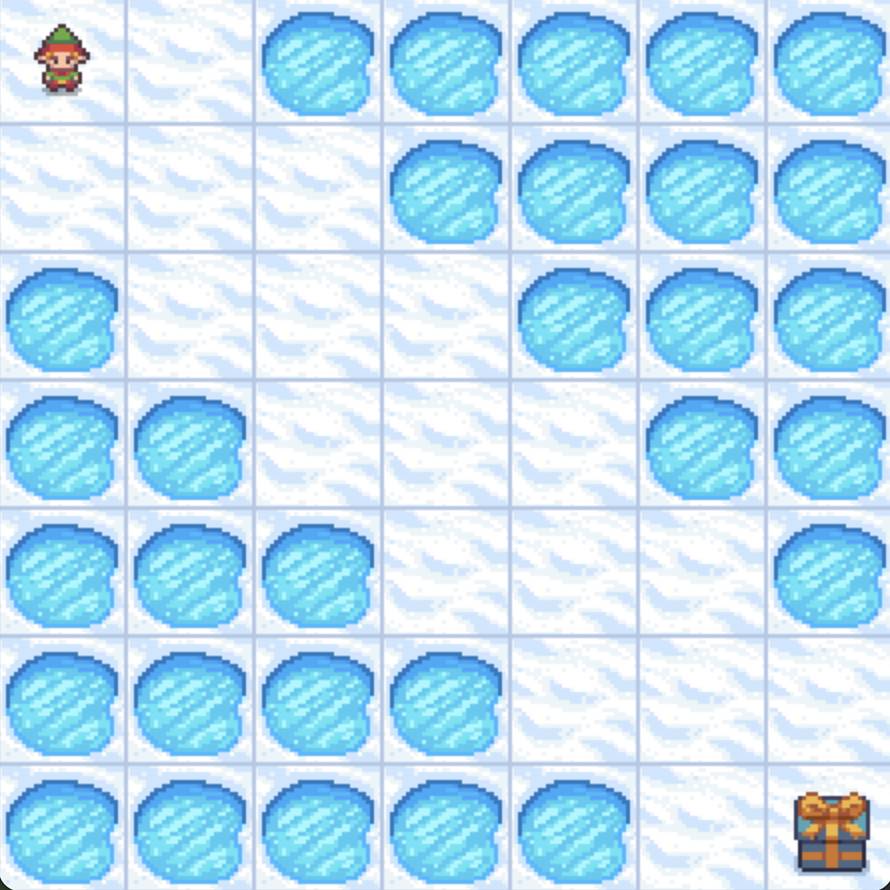
\includegraphics[width=0.8\linewidth]{Env_2.png}
        \caption{Carte — Cas 2}\label{fig:map2}
    \end{minipage}
    \hfill
    \begin{minipage}{0.32\textwidth}
        \centering
        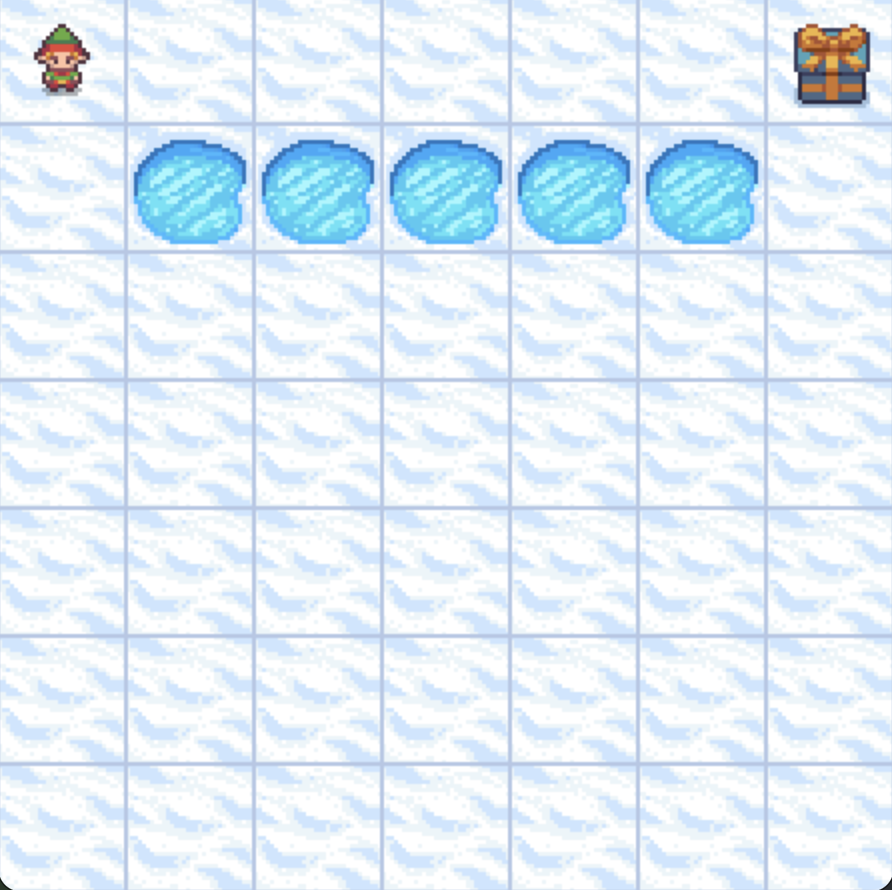
\includegraphics[width=0.8\linewidth]{Env_3.png}
        \caption{Carte — Cas 3}\label{fig:map3}
    \end{minipage}
\end{figure}

% =============================================================================
\section{Stratégies considérées}
% =============================================================================

\subsection{Stratégies de référence (baselines)}

Nous avons retenu deux stratégies tabulaires basées sur les différences temporelles (\textit{TD learning}), qui ne comportent aucun mécanisme explicite d'évitement des situations dangereuses.

\textbf{Q-learning (off-policy)} \citep{watkins1989qlearning} apprend la fonction de valeur d'action optimale $Q^*(s, a)$ indépendamment de la politique d'exploration. La règle de mise à jour est :
\begin{equation}
Q(S_t, A_t) \leftarrow Q(S_t, A_t) + \alpha \left[ R_{t+1} + \gamma \max_{a} Q(S_{t+1}, a) - Q(S_t, A_t) \right]
\label{eq:qlearning}
\end{equation}
La cible utilise le \textit{maximum} sur les actions suivantes, ce qui revient à supposer que l'agent agira de manière optimale à l'avenir. Cette hypothèse rend Q-learning optimiste face au risque : il évalue les actions en ignorant le coût réel de son comportement exploratoire.

\textbf{SARSA (on-policy)} \citep{rummery1994sarsa} apprend la valeur de la politique effectivement exécutée, en utilisant l'action $A_{t+1}$ réellement choisie par la politique d'exploration :
\begin{equation}
Q(S_t, A_t) \leftarrow Q(S_t, A_t) + \alpha \left[ R_{t+1} + \gamma Q(S_{t+1}, A_{t+1}) - Q(S_t, A_t) \right]
\label{eq:sarsa}
\end{equation}
Puisque $A_{t+1}$ est sélectionnée selon la politique $\epsilon$-greedy (qui peut choisir des actions sous-optimales ou dangereuses), SARSA intègre le risque inhérent à l'exploration dans ses estimations, conduisant à des politiques plus prudentes.

\subsection{Survol des stratégies adaptées}

Trois approches de la littérature ont été identifiées comme spécifiquement conçues pour réduire les situations dangereuses pendant l'apprentissage.

\textbf{Q-learning sensible au risque} \citep{mihatsch2002risksensitive} modifie la mise à jour TD par une transformation asymétrique de l'erreur : les erreurs négatives (mauvaises surprises) sont sur-pondérées par rapport aux positives via un paramètre $\kappa \in (-1, 1)$. Cette approche reste tabulaire et converge vers une politique \textit{risk-sensitive} dont les propriétés théoriques sont établies. Lorsque $\kappa \to 0$, la méthode se réduit au Q-learning standard, ce qui en fait une généralisation directe et rétrocompatible des baselines.

\textbf{RL sensible au risque de défaillance} \citep{geibel2005risksensitive} définit le risque comme la probabilité d'atteindre un état erroné, et modifie la fonction de valeur pour minimiser directement cette probabilité. Cette probabilité est estimée via un opérateur de Bellman modifié qui propage la dangerosité des états terminaux négatifs vers les états voisins. L'approche requiert une étiquette explicite des états dangereux (ici les tuiles H), mais offre des garanties théoriques de convergence vers une politique minimisant le taux de défaillance. Elle est particulièrement adaptée aux environnements où les états négatifs sont clairement identifiables et statiques, comme FrozenLake.

\textbf{Safe RL par exploration sûre} \citep{moldovan2012safe} propose une approche basée sur l'ergodicité des politiques : l'agent n'est autorisé à exécuter que des actions depuis lesquelles il lui est garanti de pouvoir revenir à un état sûr de départ. Cette contrainte élimine structurellement les états terminaux négatifs durant l'exploration, au prix d'une planification supplémentaire à chaque pas. La vérification d'ergodicité nécessite de connaître les probabilités de transition, ce qui suppose un modèle de l'environnement disponible ou estimé.

\subsection{Stratégie prometteuse : Q-learning sensible au risque}

Nous avons sélectionné le \textbf{Q-learning sensible au risque} \citep{mihatsch2002risksensitive} comme stratégie prometteuse. Son principal avantage est d'être directement comparable aux baselines tabulaires tout en introduisant un mécanisme explicite de prise en compte du risque. La transformation asymétrique de l'erreur TD est définie par :
\begin{equation}
f_\kappa(\delta) =
\begin{cases}
(1 + \kappa)\,\delta & \text{si } \delta \geq 0 \\
(1 - \kappa)\,\delta & \text{si } \delta < 0
\end{cases}
\label{eq:risktransform}
\end{equation}
où $\delta = R_{t+1} + \gamma \max_a Q(S_{t+1}, a) - Q(S_t, A_t)$ est l'erreur TD standard. La mise à jour devient :
\begin{equation}
Q(S_t, A_t) \leftarrow Q(S_t, A_t) + \alpha\, f_\kappa(\delta)
\label{eq:riskql}
\end{equation}
Avec $\kappa < 0$ (mode \textit{risk-averse}), les erreurs négatives sont amplifiées d'un facteur $(1 - \kappa) > 1$, rendant l'agent plus sensible aux pénalités et l'incitant à éviter les situations pouvant conduire à une chute. Par rapport à l'approche de Geibel \& Wysotzki (\citeyear{geibel2005risksensitive}) qui nécessite une définition explicite des états dangereux, cette méthode s'adapte automatiquement via les récompenses de l'environnement.

% =============================================================================
\section{Méthodologie expérimentale}
% =============================================================================

\subsection{Implémentation}

Les trois stratégies sont tabulaires : les tables $Q$ et les politiques d'exploration sont implémentées avec \textbf{NumPy}~\citep{numpy}, et les environnements sont générés via \textbf{Gymnasium}~\citep{towers2024gymnasium}. Le code source est intégralement documenté (docstrings, commentaires inline) et disponible sur le dépôt GitHub du projet.

\subsection{Hyperparamètres}

Les hyperparamètres communs aux trois stratégies sont : taux d'apprentissage $\alpha = 0.1$, facteur d'escompte $\gamma = 0.99$, exploration $\epsilon$-greedy avec décroissance exponentielle $\epsilon(t) = \max(0.9995^{t-1},\; 0.01)$. Ces valeurs suivent les recommandations standard de la littérature tabulaire~\citep{rlbook} et ont été validées par essais préliminaires sur le Cas~1. Pour le Q-learning sensible au risque, le paramètre de risque est fixé à $\kappa = -0.5$ : cette valeur a été sélectionnée par recherche sur la grille $\kappa \in \{-0.25, -0.5, -0.75\}$, en retenant la valeur offrant la plus forte réduction des chutes sur l'ensemble des cas d'étude.

\subsection{Paramètres expérimentaux}

Chaque stratégie est entraînée sur \textbf{100~000 épisodes} par cas d'étude. La longueur maximale d'un épisode est de \textbf{100 pas}. Les expériences sont répétées sur \textbf{5 graines aléatoires} pour obtenir des estimations stables. L'évaluation finale est réalisée en mode greedy (sans exploration) sur \textbf{1~000 épisodes} distincts de l'entraînement.

\subsection{Indicateurs de performance}

\begin{enumerate}[noitemsep, topsep=0pt]
    \item \textbf{Récompense cumulative moyenne} : indicateur global combinant gains (objectif) et pénalités (chutes, pas).
    \item \textbf{Taux de chute} : proportion d'épisodes terminant sur une tuile H — indicateur central de la sécurité.
    \item \textbf{Taux de succès} : proportion d'épisodes atteignant la tuile G — indicateur de l'efficacité de la politique finale.
    \item \textbf{Évolution du taux de chute pendant l'entraînement} : permet de mesurer si une stratégie réduit le nombre de situations dangereuses \textit{au cours} de l'apprentissage, pas seulement en évaluation finale.
\end{enumerate}

% =============================================================================
\section{Résultats}
% =============================================================================

Le Tableau~\ref{tab:comparaison} présente les métriques d'évaluation greedy (moyennes sur 5 seeds). Plusieurs observations sont à noter.

\textbf{Cas 1.} Les trois stratégies convergent vers des performances équivalentes ($\approx$95\% de succès), ce qui est attendu dans un environnement peu dangereux : le mécanisme de sensibilité au risque n'apporte pas de bénéfice mesurable.

\textbf{Cas 2.} Le Q-learning sensible au risque réduit spectaculairement le taux de chute à \textbf{0.1\%} en évaluation, contre 17--18\% pour les baselines. Cependant, son taux de succès est lui aussi proche de zéro : l'agent a appris à ne pas s'aventurer dans le couloir dangereux, atteignant rarement l'objectif. Ce phénomène de \textit{paralysie} illustre les limites d'une aversion au risque non contrainte.

\textbf{Note sur les taux de chute comparables entre les cas 2 et 3.} Q-learning présente des taux de chute similaires en Cas~2 (15.6\%) et en Cas~3 (17.3\%), mais son taux de succès est très différent (57.4\% contre 82.5\%). Cette différence s'explique par la structure des environnements : en Cas~2, le couloir diagonal étroit implique que les épisodes sans chute se terminent fréquemment par un timeout — l'agent glisse hors de la trajectoire praticable sans forcément tomber dans un trou, puis erre jusqu'à la limite de 100 pas sans atteindre l'objectif. En Cas~3, la grille est beaucoup plus ouverte : un épisode qui évite les trous débouche presque inévitablement sur l'objectif.

\textbf{Cas 3.} Le résultat est contre-intuitif : le Q-learning sensible au risque obtient le \textit{pire} taux de chute (53.9\%), nettement supérieur aux baselines. La déformation asymétrique de la table $Q$ conduit l'agent vers un comportement pathologique dans un environnement où la récompense de l'objectif est élevée mais les pénalités de pas sont aussi amplifiées.

\textbf{Note sur les récompenses moyennes.} Les récompenses du Tableau~\ref{tab:comparaison} ne sont pas directement comparables entre cas, car les \textit{reward\_schedule} diffèrent. En particulier, le cas 3 utilise une récompense d'objectif de $+1.75$ (vs $+1.0$ pour les cas 1 et 2) mais aussi une pénalité par pas de $-0.05$, ce qui réduit significativement la récompense cumulative même pour les épisodes couronnés de succès. Ainsi, un taux de succès élevé (82.1\% pour Q-learning en cas 3) peut coexister avec une récompense moyenne modeste (0.19) du fait des pénalités accumulées sur chaque pas.

\begin{table}[ht]
\centering
\small
\begin{tabular}{llccc}
\toprule
\textbf{Cas d'étude} & \textbf{Stratégie} & \textbf{Récompense moy.} & \textbf{Taux de chute} & \textbf{Taux de succès} \\
\midrule
\multirow{3}{*}{Cas 1 : Efficacité}
  & Q-learning              & $0.768 \pm 0.056$ & $4.0 \pm 2.1$\%  & $95.8 \pm 1.7$\% \\
  & SARSA                   & $0.788 \pm 0.011$ & $5.5 \pm 0.8$\%  & $94.5 \pm 0.8$\% \\
  & Q-l. sensible au risque & $0.794 \pm 0.004$ & $5.3 \pm 0.3$\%  & $94.7 \pm 0.3$\% \\
\midrule
\multirow{3}{*}{Cas 2 : Évitement}
  & Q-learning              & $0.418 \pm 0.210$ & $15.6 \pm 8.2$\% & $57.4 \pm 28.8$\% \\
  & SARSA                   & $0.419 \pm 0.163$ & $18.6 \pm 8.6$\% & $60.5 \pm 23.4$\% \\
  & Q-l. sensible au risque & $0.000 \pm 0.002$ & $\mathbf{0.1 \pm 0.1}$\% & $0.1 \pm 0.2$\% \\
\midrule
\multirow{3}{*}{Cas 3 : Compromis}
  & Q-learning              & $0.206 \pm 0.016$ & $17.3 \pm 1.9$\% & $82.5 \pm 1.9$\% \\
  & SARSA                   & $0.060 \pm 0.147$ & $23.1 \pm 15.9$\%& $76.8 \pm 15.8$\% \\
  & Q-l. sensible au risque & $0.006 \pm 0.075$ & $\mathbf{53.9 \pm 4.1}$\% & $46.1 \pm 4.1$\% \\
\bottomrule
\end{tabular}
\vspace{0.2em}
\caption{Performances des stratégies en évaluation greedy (moyenne $\pm$ écart-type sur 5 seeds, 1~000 épisodes).}
\label{tab:comparaison}
\end{table}

Les Figures~\ref{fig:rewards} et~\ref{fig:holes} montrent l'évolution pendant l'entraînement (lissée sur une fenêtre de 500 épisodes). En Cas~2, le Q-learning sensible au risque maintient un taux de chute quasi-nul dès les premiers épisodes — bien inférieur aux baselines — ce qui confirme que le mécanisme opère pendant l'apprentissage et pas uniquement en évaluation. En Cas~3, les trois stratégies présentent des taux de chute élevés en début d'entraînement (phase d'exploration), puis divergent : SARSA et le Q-l. sensible au risque restent à des niveaux élevés tandis que Q-learning converge vers un taux plus faible.

\begin{figure}[H]
    \centering
    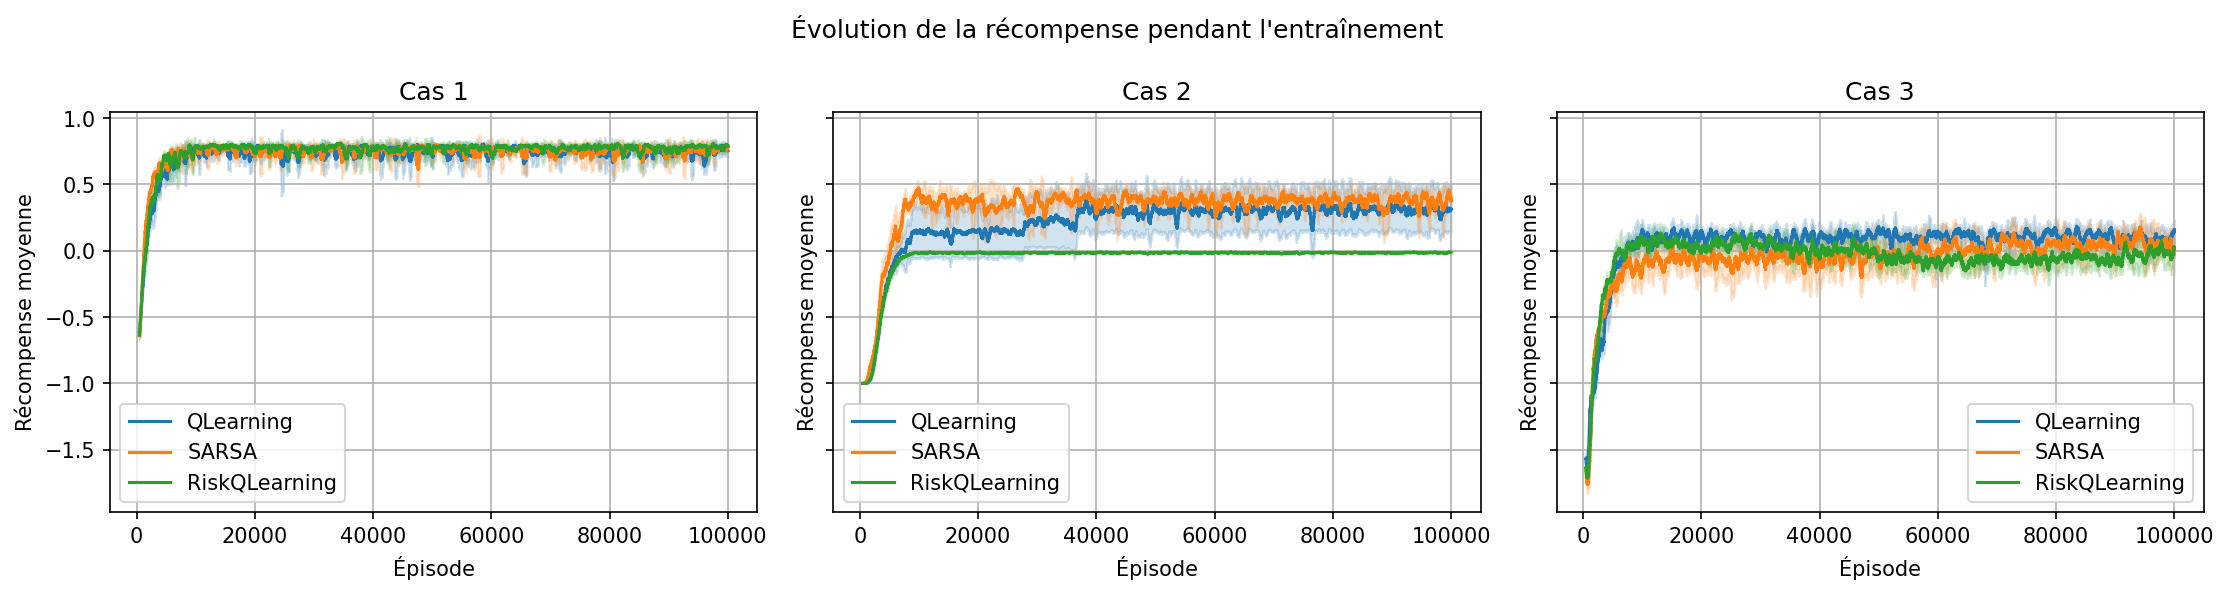
\includegraphics[width=1\linewidth]{rewards.png}
    \caption{Évolution de la récompense moyenne pendant l'entraînement (lissage 500 épisodes, moyenne $\pm$ écart-type sur 5 seeds). L'axe Y est partagé entre les cas pour permettre la comparaison.}
    \label{fig:rewards}
\end{figure}

\begin{figure}[H]
    \centering
    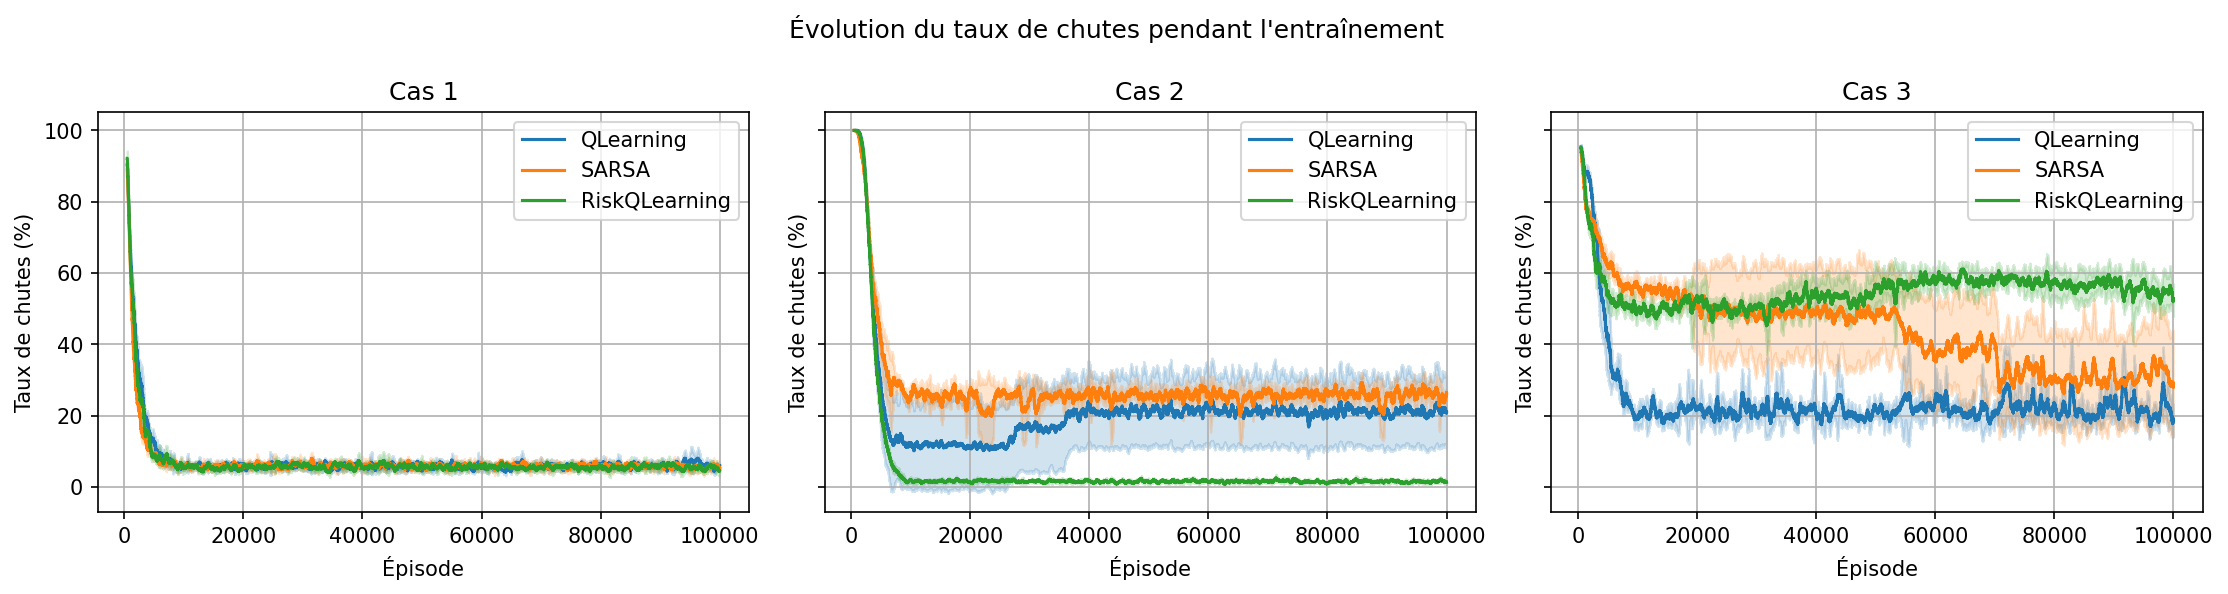
\includegraphics[width=1\linewidth]{holes.png}
    \caption{Évolution du taux de chutes pendant l'entraînement (lissage 500 épisodes, moyenne $\pm$ écart-type sur 5 seeds). En Cas~2, le Q-l. sensible au risque réduit quasi-immédiatement les chutes.}
    \label{fig:holes}
\end{figure}

% =============================================================================
\section{Discussion}
% =============================================================================

\subsection{Liens avec la littérature et explication des résultats}

Les résultats obtenus sont cohérents avec les prédictions théoriques de la littérature. La différence fondamentale entre Q-learning (off-policy) et SARSA (on-policy) se manifeste clairement dans les cas 2 et 3. Comme décrit par \citet{rlbook}, Q-learning converge vers la politique optimale au sens de la récompense espérée, sans égard pour les conséquences de son comportement exploratoire. SARSA, en revanche, évalue la politique qu'il exécute réellement, ce qui l'amène à développer une certaine prudence dans les zones à haut risque. C'est ce qui explique que SARSA obtient un meilleur taux de succès en Cas~2 (60.5\% vs 57.4\%) : sa prudence pendant l'entraînement lui permet de maîtriser un couloir où chaque glissade est fatale.

Le comportement du Q-learning sensible au risque \citep{mihatsch2002risksensitive} révèle une tension fondamentale entre sécurité et efficacité. En Cas~2, l'amplification des erreurs TD négatives conduit l'agent à fuir toute zone pouvant mener à une pénalité. La politique apprise évite effectivement les trous, mais elle évite aussi de s'approcher de l'objectif. Ce phénomène — que l'on peut qualifier de \textit{paralysie par aversion au risque} — est une limite connue des méthodes de safe RL : une contrainte de sécurité sans borne inférieure sur la performance peut conduire à une politique triviale (ne jamais bouger), comme le notent \citet{moldovan2012safe} en discutant des limites de l'exploration sûre par ergodicité.

En Cas~3, le comportement contre-intuitif du Q-learning sensible au risque s'explique par l'interaction entre la transformation asymétrique et la structure des récompenses. La forte récompense de l'objectif ($+1.75$) est atténuée d'un facteur $(1+\kappa) = 0.5$ dans la mise à jour, tandis que la pénalité de chute ($-1.0$) est amplifiée d'un facteur $(1-\kappa) = 1.5$. Mais la pénalité par pas ($-0.05$) est également amplifiée, créant une forte pression pour terminer rapidement les épisodes. L'agent converge vers le chemin court (6~pas) car la pénalité cumulative du long chemin (18~pas $\times$ 0.075 amplifiés = 1.35 de perte) dépasse la pénalité de chute amplifiée (1.5). Cette déformation de la surface des valeurs conduit à plus de chutes que les baselines, illustrant que la sensibilité au risque mal calibrée peut être contre-productive.

\subsection{Réflexion sur les approches}

Du point de vue de la \textbf{complexité algorithmique}, les trois stratégies sont identiques : $O(|\mathcal{S}| \times |\mathcal{A}|)$ en espace mémoire et $O(1)$ par mise à jour. Le Q-learning sensible au risque n'introduit qu'une opération supplémentaire par pas de temps (le calcul de $f_\kappa$), sans surcoût notable.

Du point de vue de l'\textbf{implémentation}, la stratégie de \citet{mihatsch2002risksensitive} est la plus simple à intégrer dans un pipeline existant : il suffit de modifier la règle de mise à jour avec un unique hyperparamètre $\kappa$. Les approches par MDP contraint (e.g., Lagrangiens) nécessiteraient une table supplémentaire et un processus d'optimisation dual, ce qui complique significativement l'implémentation et le réglage.

La \textbf{sensibilité aux hyperparamètres} est cependant un défi majeur de la méthode : la valeur optimale de $\kappa$ dépend fortement de la structure des récompenses. Nos résultats montrent qu'une même valeur ($\kappa = -0.5$) peut éliminer quasi totalement les chutes en Cas~2 tout en les aggravant dramatiquement en Cas~3.

\subsection{Message général au client}

Notre étude révèle que les stratégies d'apprentissage par renforcement standard (Q-learning, SARSA) présentent des limites importantes dans des environnements où éviter les situations dangereuses est aussi critique que d'atteindre l'objectif. Même SARSA, qui est naturellement plus prudent que Q-learning grâce à sa nature on-policy, ne parvient pas à garantir un faible taux de chutes dans des environnements étroits et très risqués.

L'introduction d'un mécanisme explicite de sensibilité au risque (ici, la transformation asymétrique de l'erreur TD) permet de réduire drastiquement les incidents pendant l'apprentissage dans des scénarios d'évitement strict. Cependant, elle peut se révéler contre-productive dans des environnements présentant un compromis explicite entre risque et récompense.

Notre recommandation pour le client est la suivante : dans des applications où les situations dangereuses ont un coût très élevé et où il existe un chemin clairement sûr vers l'objectif, le Q-learning sensible au risque offre des garanties de sécurité pendant l'apprentissage que les méthodes standards ne peuvent pas offrir. Cependant, si l'environnement impose un compromis inévitable entre efficacité et sécurité, le calibrage de $\kappa$ doit être réalisé avec soin, idéalement sur un simulateur avant tout déploiement réel. Dans ce contexte, il convient d'explorer des approches plus sophistiquées — comme les MDP contraints — qui permettent de fixer explicitement un seuil maximal de taux de chutes comme contrainte dure.

% =============================================================================
% BIBLIOGRAPHY
% =============================================================================
\newpage
\begin{thebibliography}{99}

\bibitem[Sutton and Barto(2018)]{rlbook}
Richard S. Sutton and Andrew G. Barto.
\newblock \textit{Reinforcement Learning: An Introduction}.
\newblock MIT Press, 2018.

\bibitem[Watkins(1989)]{watkins1989qlearning}
Christopher J. C. H. Watkins.
\newblock Learning from delayed rewards.
\newblock PhD thesis, University of Cambridge, 1989.

\bibitem[Rummery and Niranjan(1994)]{rummery1994sarsa}
Gavin A. Rummery and Mahesan Niranjan.
\newblock On-line Q-learning using connectionist systems.
\newblock Technical Report CUED/F-INFENG/TR 166, University of Cambridge, 1994.

\bibitem[Mihatsch and Neuneier(2002)]{mihatsch2002risksensitive}
Oliver Mihatsch and Ralph Neuneier.
\newblock Risk-sensitive reinforcement learning.
\newblock \textit{Machine Learning}, 49:267--290, 2002.

\bibitem[Geibel and Wysotzki(2005)]{geibel2005risksensitive}
Peter Geibel and Fritz Wysotzki.
\newblock Risk-sensitive reinforcement learning applied to control under constraints.
\newblock \textit{Journal of Artificial Intelligence Research}, 24:81--108, 2005.

\bibitem[Moldovan and Abbeel(2012)]{moldovan2012safe}
Teodor M. Moldovan and Pieter Abbeel.
\newblock Safe exploration in Markov decision processes.
\newblock In \textit{Proceedings of the 29th International Conference on Machine Learning (ICML)}, pages 1451--1458, 2012.

\bibitem[Harris et al.(2020)]{numpy}
Charles R. Harris et al.
\newblock Array programming with {NumPy}.
\newblock \textit{Nature}, 585:357--362, 2020.

\bibitem[Towers et al.(2024)]{towers2024gymnasium}
Mark Towers et al.
\newblock Gymnasium: A standard interface for reinforcement learning environments.
\newblock \textit{arXiv preprint arXiv:2407.17032}, 2024.

\end{thebibliography}

\end{document}
